\documentclass{article}
\setlength{\parskip}{5pt} % esp. entre parrafos
\setlength{\parindent}{0pt} % esp. al inicio de un parrafo
\usepackage{amsmath} % mates
\usepackage[sort&compress,numbers]{natbib} % referencias
\usepackage{url} % que las URLs se vean lindos
\usepackage[top=25mm,left=20mm,right=20mm,bottom=25mm]{geometry} % margenes
\usepackage{hyperref} % ligas de URLs
\usepackage{graphicx} % poner figuras
\usepackage[spanish]{babel} % otros idiomas

\author{Raul Lagunes Rivera \\\\2125677} % author
\title{Pr\'{a}ctica 1 Movimiento Browniano}%titulo
\date{\today}

\begin{document} % inicia contenido

\maketitle % cabecera


\section{Introducci\'{o}n}\label{intro} % seccion y etiqueta



La  pr\'{a}ctica n\'{u}mero 1  estudia el tema Movimiento Browniano, donde se debe analizar el tiempo de regreso al origen de dicha part\'{i}cula en 5 dimenciones , variando el n\'{u}mero de pasos de la caminata, con 30 repeticiones del experimento para cada combinaci\'{o}n\citep{ejemplo}.

\section{Objetivo}
El objetivo de la simulaci\'{o}n es examinar de manera sistem\'{a}tica los efectos de la dimensi\'{o}n en la distancia Euclideana m\'{a}xima del origen del movimiento browniano para cinco dimenciones, variando el n\'{u}mero de pasos de la caminata (100,1000,10000 pasos), con 30 repeticiones del experimento para cada combinacion y grafica los resultados en una sola figura diagrama caja-bigote


\section{C\'{o}digo}
En el siguiente c\'{o}digo se utilizaron secuencias for para realizar todo el objetivo propuesto en una sola ejecución.El c\'{o}digo base se sac\'{o} del repertorio de la Dra. Elisa Schaeffer.
\\ Codigo en phyton 
\\\url{https://github.com/satuelisa/Simulation/blob/master/BrownianMotion}\\
**Código creado en Python**\
\begin{verbatim}
from random import random, randint
from math import fabs, sqrt
import matplotlib.pyplot as plt
import numpy as np 
DIMS=1,2,3,4,5  cuantas dimenciones
caminatas= 100, 1000, 10000
replicas = 30  cuantas veces
CB_100=[]
CB_1000=[]
CB_10000=[]
for dim in DIMS:
    print("######### Dimencion:",dim,"###########################")
    cien=[]
    mil=[]
    diezmill=[]
    for replica in range (replicas):
        pos=[0]* dim
        mayor= 0
        re=0
        mayores=[]
        for s in caminatas:
            for paso in range(s):
                eje= randint(0, dim - 1)
                if random()< 0.5:
                    pos[eje] +=1
                else:
                    pos[eje]-= 1
                mayor = max ( mayor, sqrt(sum([p**2 for p in pos])))
            mayores.append(mayor)
        cien.append(mayores[0])
        mil.append(mayores[1])
        diezmill.append(mayores[2])
        CB_100.append(cien)
    CB_1000.append(mil)
    CB_10000.append(diezmill)
    
print("cuantos datos de caja bigote",len(CB_100))
pb=plt.boxplot([CB_100[0],CB_1000[0],CB_10000[0],CB_100[1],
CB_1000[1],CB_10000[1],CB_100[2],CB_1000[2],CB_10000[2],
CB_100[3],CB_1000[3],CB_10000[3],CB_100[4],CB_1000[4],CB_10000[4]])
plt.xticks([1,2,3,4,5,6,7,8,9,10,11,12,13,14,15],
         ['100','1000','10000','100','1000','10000',
         '100','1000','10000','100','1000','10000','100','1000','10000'])

plt.xlabel('camintas')
plt.ylabel('Distancia máxima')
plt.tick_params(axis='x', rotation=45)
plt.title('Distancia Euclidiana')


colors = ['orange','orange','orange','red','red', 'red',   
          'green','green','green', 'pink','pink','pink','blue','blue','blue']

for patch, color in zip(pb['boxes'], colors): 
    patch.set_color(color)
    
plt.plot([], c='orange', label='dimencion 1')
plt.plot([], c='red', label='dimencion 2')
plt.plot([], c='green', label='dimencion 3')
plt.plot([], c='pink', label='dimencion 4 ')
plt.plot([], c='blue', label='dimencion 5')

plt.legend()
    
plt.savefig('figuraPy.png') # mandar a un archivos

        
print(pos)

\end{verbatim}






\newpage

% Computational Results
\section{Resultados}
En la figura se muestra como se comporta cada dimencion con diferente tamaño de camina , de color amarillo es la dimension uno y sus tres respectivas caminas, y asi sucesivamente con las sinco dimensiones.


 \begin{figure}[h]
     \centering
     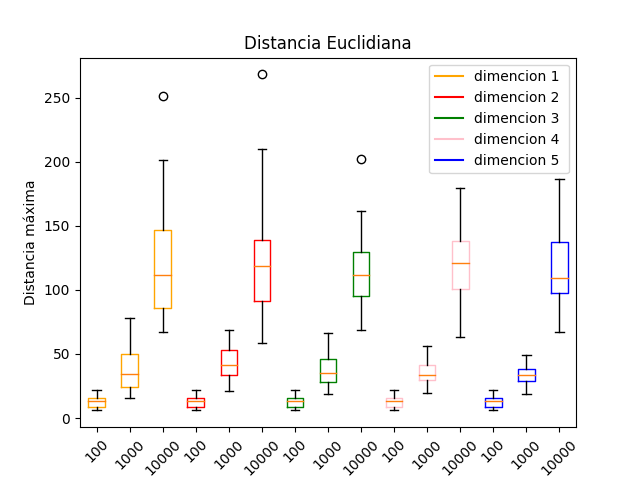
\includegraphics[width=100mm]{imagenes/figuraPy.png}
        \caption{tomado del repositorio de Raul Lagunes Rivera del codigo de python 
    \url{https://github.com/Raullr28/Resultados/blob/main/P1/figuraPy.png}}
     \label{}
 \end{figure}




 
 \section{Conclusiones}

 se realizo la tarea numero 1 correctamente ,obteniendo la caja-bigote esperada con las caminas propuestas y las dimensiones deseadas 
 
 \bibliography{biblio.bib}
 \bibliographystyle{plainnat}

 \end{document}
